\chapter{Linear Algebra II}

\newpage

% Gamla tentor
% https://www.studocu.com/sv/document/uppsala-universitet/linjaer-algebra-ii/gamla-tentor/tenta-oktober-2018-fragor/6649302/view
% https://www.studocu.com/sv/document/uppsala-universitet/linjaer-algebra-ii/gamla-tentor/tenta-mars-2016-fragor/3544944/view


\begin{multicols}{2}
\section{Grudläggande teori} % grunden
\subsection{Ekvationssystem och matris räkning}
\begin{align*}
  &\quad \left\{\begin{array}{rr}
  x+2 y+ & z=-1 \\
  2 x+(a+3) y+ & 3 z=-4 \\
  x+(3-a) y+(a-2) z & =a-1
  \end{array}\right. \\
  &\quad \left(\begin{array}{ccc|c}
    1 & 2 & 1 & -1 \\
    2 & a+3 & 3 & -4 \\
    1 & 3-a & a-2 & a-1
  \end{array}\right) \\
  &\quad (-1 \text{ rad1 till rad2}), (-2 \text{ rad1 till rad3}) \\
  &\quad \left(\begin{array}{ccc|c}
    1 & 2 & 1 & -1 \\
    2 & a-1 & 1 & -2 \\
    0 & 1-a & a-3 & a
  \end{array}\right) \\
  &\quad \left(\begin{array}{ccc|c}
    1 & 2 & 1 & -1 \\
    0 & a-1 & 1 & -2 \\
    0 & 0 & a-2 & a-2
  \end{array}\right) \\
  &\quad a \neq 1 \land a \neq 2 \\
  &\quad (\frac{1}{a-2} \text{rad 3}) \\
  &\quad \left(\begin{array}{ccc|c}
    1 & 2 & 1 & -1 \\
    0 & a-1 & 1 & -2 \\
    0 & 0 & 1 & 1
  \end{array}\right) \\
  &\quad (-1 \text{rad 3 till rad 2}), (-1 \text{rad 3 till rad 1}) \\
  &\quad \left(\begin{array}{ccc|c}
    1 & 2 & 0 & -2 \\
    0 & a-1 & 0 & -3 \\
    0 & 0 & 1 & 1
  \end{array}\right) \\
  &\quad (\frac{1}{a-1} \text{rad 2}) \\
  &\quad \left(\begin{array}{ccc|c}
    1 & 2 & 0 & -2 \\
    0 & a-1 & 0 & -3 \\
    0 & 0 & 1 & 1
  \end{array}\right) \\
  &\quad \left(\begin{array}{ccc|c}
    1 & 2 & 0 & -2 \\
    0 & 1 & 0 & \frac{3}{1-a} \\
    0 & 0 & 1 & 1
  \end{array}\right) \\  
  &\quad (-2 \text{rad 2 till rad 3}) \\
  &\quad \left(\begin{array}{ccc|c}
    1 & 0 & 0 & -2 - \frac{6}{1-a} \\
    0 & 1 & 0 & \frac{3}{1-a} \\
    0 & 0 & 1 & 1
  \end{array}\right) \\  
  &\quad \left\{\begin{array}{rr}
  x & = -2 - \frac{6}{1-a} \\
  y & = \frac{3}{1-a} \\
  z & = 1
  \end{array}\right. \\
  &\quad \\
  &\quad \text{\textbf{Kontroll:} stoppar in x,y,z i ekvationerna} \\
  &\quad \left\{\begin{array}{r}
  \left(\frac{2 a-8}{1-a}\right)+\quad 2 \cdot\left(\frac{3}{1-a}\right)+\quad 1=-1 \\
  2 \cdot\left(\frac{2 a-8}{1-a}\right)+(a+3) \cdot\left(\frac{3}{1-a}\right)+\quad 3 \cdot 1=-4 \\
  \left(\frac{2 a-8}{1-a}\right)+(3-a) \cdot\left(\frac{3}{1-a}\right)+(a-2) \cdot 1=a-1
  \end{array}\right.
\end{align*}


\subsection{determinanter}
\begin{align*}
  &\left(\begin{array}{cccc}
    1   & x   & x^2 & x^3  \\
    1   & x^2 & x^3 & x^4  \\
    x   & x^2 & x^4 & x^5  \\
    x^2 & x^3 & x^4 & x^6  \\
  \end{array}\right) \\
  &\\
  &x
  \left(\begin{array}{cccc}
    1   & x   & x^2 & x^3  \\
    1   & x^2 & x^3 & x^4  \\
    1   & x   & x^3 & x^4  \\
    x^2 & x^3 & x^4 & x^6  \\
  \end{array}\right) \\
  &= \text{rad 4 -rad 1} x^3  
  \left(\begin{array}{cccc}
    1   & x   & x^2 & x^3  \\
    1   & x^2 & x^3 & x^4  \\
    1   & x   & x^3 & x^4  \\
    1   & x   & x^2 & x^4  \\
  \end{array}\right) \\
  &=  x^3
  \left(\begin{array}{cccc}
    1   & x   & x^2 & x^3  \\
    1   & x^2 & x^3 & x^4  \\
    1   & x   & x^3 & x^4  \\
    0   & 0   & 0 & x     \\
  \end{array}\right)^{R4}  \\
  &= \text{rad 3 -rad 1} x^3(x^4-x^3)
  \left(\begin{array}{ccc}
    1   & x   & x^2  \\
    1   & x^2 & x^3  \\
    1   & x   & x^3  \\
  \end{array}\right) \\
  &= x^6(x-1)^2
  \left(\begin{array}{ccc}
    1   & x   & x^2  \\
    1   & x^2 & x^3  \\
    0   & 0   & x  \\
  \end{array}\right)  \\
  &= x^6(x-1)(x^3-x^2)  
  \left(\begin{array}{cc}
    1   & x    \\
    1   & x^2  \\
  \end{array}\right) = x^9(x-1)^3=0
\end{align*}

\subsection{flerdimisionel dvs $R^n$}
räkneregler

\subsection{Funktioner}
polynom functioner vid en viss grad också

\subsection{Linjer}
\begin{align*}
  &\quad  l: \begin{pmatrix} x \\ y \\ z \end{pmatrix} =
  \begin{pmatrix} 3 \\ 2 \\ 5 \end{pmatrix} + t\begin{pmatrix} 1 \\ 2 \\ 2 \end{pmatrix} \\
  &\quad  \text{Då är riktnings vektorn } \begin{pmatrix} 1 \\ 2 \\ 2 \end{pmatrix} \\
  &\quad  \text{Och går genom } \begin{pmatrix} 3 \\ 2 \\ 5 \end{pmatrix} \\
\end{align*}


\section{Vektorrum}
\textbf{Definition: vektor rum}
En mängd $\mathbb{V}$ kallas för en \underline{reellt vektorrum} om:\newline
1. Det finns en operator på  $\mathbb{V}$ som kallas addition och
beräknas med $+$, sådant att om $\vec{u},\vec{v} \in \mathbb{V}$ så gäller
$\vec{u}+\vec{v}\in\mathbb{V}$.\newline
2. Det finns en poeration på  $\mathbb{V}$ som kallas skalning eller
multipliseras med reella tal, som beteknas med $\cdot$, sådan
att om $\lambda\in\mathbb{R} \land \vec{v}\in\mathbb{V}$ så gäller
$\lambda\cdot\vec{v}\in\mathbb{V}$
räknereglerna gäller som i la1
%kommutitiva lag, assositiv lag ..

\textbf{Axiomen: vektor rum}
\begin{align*}
  &\quad  \text{1. } \vec{u}+\vec{v} = \vec{v}+\vec{u} \text{ (Kommutativ lag)} \\
  &\quad  \text{2. } \vec{u}(\vec{v}+\vec{w}) = (\vec{u}+\vec{v})+\vec{w} \text{ (Associativ lag)} \\
  &\quad  \text{3. } \text{Det finns ett nollement } \vec{0} \text{ så att }
  \vec{v}+\vec{0}=\vec{v} \\
  &\quad  \text{4. } \text{Till varge } \vec{v}\in\mathbb{V} \text{ finns ett element }
  -\vec{v} \text{ så att} \\
  &\quad  \vec{v}+(-\vec{v}) = 0 \\
  &\quad  \text{5. } 1\cdot\vec{v} = \vec{v} \\
  &\quad  \text{6. } \lambda\cdot(\mu\cdot\vec{v}) = (\lambda\cdot\mu)\cdot\vec{v}
  \text{ (Associativ lag)} \\
  &\quad  \text{7. } (\lambda+\mu)\cdot\vec{v} = \lambda\cdot\vec{v} + \mu\cdot\vec{v}
  \text{ (Distributiv lag)} \\
  &\quad  \text{8. } \lambda\cdot(\vec{u}+\vec{v}) = \lambda\cdot\vec{u} + \lambda\cdot\vec{v}
  \text{ (Distributiv lag)} \\
  &\quad  \forall\lambda,\mu\in\mathbb{R}\land\vec{u},\vec{v},\vec{w}\in\mathbb{V} \\
\end{align*}


\newpage

\section{Underrum och linjära höljet}
Ett underrum är en delmängd $u$ ej $0$ som är sluten under addition och skalning

\textbf{Definition: Underrum}
En delmängd $\mathbb{U}$ av ett vektorrum $\mathbb{V}$ kallas för
ett underrum eller delrum av $\mathbb{V}$ om $\mathbb{U}$ är ett vektorrum
med den additionoch den multiplikation med reella tal som definierats i
$\mathbb{V}$.

\textbf{Sats: Underrum}
\begin{align*}
  &\quad  \text{En icketom mängd $\mathbb{U}$ av ett vektorrum $\mathbb{V}$ är ett} \\
  &\quad  \text{underrum om och endast om följande gäller} \\
  &\quad  \text{1. Om } \vec{u}\in\mathbb{U} \text{ och } \vec{v}\in\mathbb{U},
  \text{ Så är } \vec{u}+\vec{v} \in\mathbb{U} \\
  &\quad  \text{2. Om } \vec{u}\in\mathbb{U} \text{ och } \lambda\in\mathbb{R},
  \text{ Så är } \lambda\vec{u} \in\mathbb{U} \\
\end{align*}

\textbf{Regler: Underrum}
\begin{enumerate}
  \item Det snabbaste sättet att testa om det gäller är om nollvektorn finns
  om den inte gör det så bryter det mot 2-lagen
  \item Homogena ekvationer och linjer/plan genonom origo gäller det alltid för
  \item Kontunerligt deriverbara, så gäller det att det är ett underrum
\end{enumerate}

\textbf{Exempel: Underrum (Ex 1)}
\begin{align*}
  &\quad  \text{är } \left\{ \begin{pmatrix} x \\ y \\ z \end{pmatrix} | x+y+z=5 \right\}
  \text{ ett underrum?} \\
  &\quad  \\
  &\quad  \text{Nej, då: } 0+0+0\neq5 \\
\end{align*} %exotisa exempel x=x^2 är ej sant då 2(1 1)^t = (2 2)^t, 2^2\neq2


\textbf{Definition: linjära höljet}
En delmängd $\mathbb{U}$ av ett vektorrum $\mathbb{V}$ kallas för
ett underrum eller delrum av $\mathbb{V}$ om $\mathbb{U}$ är ett vektorrum
med den addition och den multiplikation med reella tal som definierats i
$\mathbb{V}$.

\textbf{Exempel: Underrum (Ex 4)}
\begin{align*}
  &\text{Vilka vektrorer i $\mathbb{P}$ tillhör } u=[1, 1+x, 1+x+x^2] \\
  &\\
  &\text{Svar: } u=P_2 \text{ (eftersom) } 1\in{u}, x\in{u}, \text{ och } x^2\in{u} \\
  &\text{Då alla } a\cdot{1} + b\cdot{x} + c\cdot{x^2} \in{u} \\
  &\text{Inga plynom av grad $>2$ tillhör $u$.} \\
  &\text{Vi för kombinera det olika elementen i u med} \\
  &\text{addition och multiplication} \\
\end{align*}
% exemepl 5.3.7

\section{Linjärt \(o\)beroende}
\textbf{Ide: linjärt beronde}
\begin{align*}
  &\text{Om vektorerna kan skrivas om en linjär kombination} \\
  &\text{av det andra vektorerna} \\
  &\text{så är vektorn linjärt beroende då det inte behöver} \\
  &\text{vektorn vi får reda på beoende genom att ställa upp ekv} \\
  &x_1\vec{v_1}+x_2\vec{v_2} + \ldots{} + x_n\vec{v_n} = \vec{0} \\
  &\text{Om denna ekvation har icke triviala lösningar} \\
  &\text{(ej noll) då är den beroende} \\
\end{align*}


\textbf{Exempel: om linjärt oberonde}
\begin{align*}
  &\quad  \text{Är mängden }  \Big\{
  \begin{pmatrix} 1 \\ 2  \end{pmatrix}
  \begin{pmatrix} 2 \\ 1  \end{pmatrix} \Big\}
  \text{i $\mathbb{R}^2$ linjärt oberoende}  \\
  &\quad
  x_1\begin{pmatrix} 1 \\ 2  \end{pmatrix} +
  x_2\begin{pmatrix} 2 \\ 1  \end{pmatrix} = \vec{0} 
  \Leftrightarrow
  \left(\begin{array}{cc|c}
    1   & 2  & 0  \\
    2   & 1  & 0  \\
  \end{array}\right) \\
  &\quad  x_1=0, x_2=0 \text{Endast triviala lösningar } \\
\end{align*}

% beviset är att kom av vektor är nollvektorn så flyttar vi över så vn är komb av det andra
% linjär kobinateion kan skrivas på säät med skalär multiplication och addition av elementen/vektorerna


\section{Bas}
\textbf{Ide: Bas och Dimention}
Bas omm om vektorerna spanner upp hella spannet och det linjärt oberonde
Standard basen $\underline{e}$
Vi behöver tree vektorer för att utgöra en bas i $\mathbb{R}^3$ är
$\vec{v_1}, \vec{v_2}, \vec{v_3} \in\mathbb{R}^3$.

Dimentioner är antallet oberonde vektorer som spänner up ``rummet''
``dimentioner blir då samma som antallet element som en bas av polynom''
$\mathbb{P}_3 = a + bx^1 + cx^2 + dx^3$ har 4 dimentioner
$\mathbb{R}^3$ har 3 dimentioner
Dimentioner för matriser är $n\times m (2\times{2}-matris = dim 4)$
En bas med tre vektorer där vektorerna $\mathbb{R}^4$ ger 3 dim

\textbf{Exempel: Ta fram bas från plan}
\begin{align*}
  &\quad  \text{låt } 2x -y z = 0 \\
  &\quad  \\
  &\quad  \text{Lösning: }  x=y/2 -z/2 \\
  &\quad  \text{Låt } y=s, \, z=t \text{ vi får då lösningen på parameter form} \\
  &\quad  \begin{pmatrix} x \\ y \\ z \end{pmatrix} =
  \begin{pmatrix} s/2 -t/2 \\ s \\ t \end{pmatrix} =
  s/2\begin{pmatrix} 1 \\ 2 \\ 0 \end{pmatrix} +
  t/2\begin{pmatrix} -1 \\ 0 \\ 2 \end{pmatrix} \\
  &\quad  \text{Basen blir då }
  \left( \begin{pmatrix} 1 \\ 2 \\ 0 \end{pmatrix} \begin{pmatrix} -1 \\ 0 \\ 2 \end{pmatrix} \right) \\
\end{align*}


\section{Basomvandling}
Vi kan ta inversen av matrisen av vektorerna som utger en bas och få
matrisen som kan multipliseras med vektor för att få omvandlingen.

\textbf{Sats: basbyte}
\begin{align*}
  &\quad  \vec{v}_{\underline{e}} = Tv_{f} \text{ Där T är en matris} \\
  &\quad  T^{\underline{f}}_{\underline{e}} = {(T^{\underline{e}}_{\underline{f}})}^{-1} \\
  &\quad  \vec{v}_{\underline{f}} = T^{\underline{e}}_{\underline{f}} \, \vec{v}_{\underline{e}} \\
\end{align*}

\textbf{Exempel: Från standar till annan bas}
\begin{align*}
  &\text{Låt } \underline{f}=(f_1 \, f_2) =
  \left( \begin{pmatrix} 2 \\ 1 \\ 1 \end{pmatrix} \begin{pmatrix} 1 \\ 2 \\ 1 \end{pmatrix} \right), \,
  \vec{v} = \begin{pmatrix} -2 \\ 5 \\ 1 \end{pmatrix} \\
  &\text{Utryck $\vec{v}$ i basen $\underline{f}$} \\
  &\\
  &\vec{v}_{\underline{e}} = \begin{pmatrix} -2 \\ 5 \\ 1 \end{pmatrix} =
  x_1 \begin{pmatrix} 2 \\ 1 \\ 1 \end{pmatrix}  + x_2 \begin{pmatrix} 1 \\ 2 \\ 1 \end{pmatrix} \\
  &\left\{\begin{array}{rr}
  2x_1 + x_2 = -2 \\
  x_1 + 2x_2 = 5  \\
  x_1 + x_2 = 1   \\
  \end{array}\right. \Rightarrow{}
  \left(\begin{array}{cc|c}
    2 & 1 & -2   \\
    1 & 2 &  5  \\
    1 & 1 &  1  \\
  \end{array}\right) \\
  &\sim{}
  \left(\begin{array}{cc|c}
    2 & 1 & -2   \\
    0 & 1 &  4  \\
    0 & 0 &  0  \\
  \end{array}\right)  \\
  &x_2 = 4, \, x_1 = 1/2(-2 -4) = -3 \Rightarrow{} 
  v_{\underline{f}} = \begin{pmatrix} -3 \\ 4 \end{pmatrix} \\
\end{align*}

\textbf{Exempel: Finn matrisen för bas byte vektorer} % polynom och vektorer
\begin{align*}
  &\quad  \text{Låt } \underline{f} =
  \left( \begin{pmatrix} 1 \\ 1 \end{pmatrix} \begin{pmatrix} 2 \\ 1 \end{pmatrix} \right)
  \text{Bestäm bas omvandling matrisen }   \\
  &\quad  \\
  &\quad  \text{Lös } T^{\underline{e}}_{\underline{f}} = 
  \left(\begin{array}{cc|cc}
    1 & 2 & 1 & 0  \\
    1 & 1 & 0 & 1  \\
  \end{array}\right) \sim
    \left(\begin{array}{cc|cc}
    1 & 0 & -1 &  2  \\
    0 & 1 &  1 & -1  \\
  \end{array}\right) \\
\end{align*}

\textbf{Exempel: Finn matrisen för bas byte polynom}
\begin{align*}
  &\quad  \text{Låt } \underline{e}=(1 \, x) \text{ och } \underline{f}=(1 \, 1-x) \\
  &\quad  \\
  &\quad  \vec{f}_1 = 1 = \vec{e}_1 \Rightarrow \vec{f_1}_e = \begin{pmatrix} 1 \\ 0 \end{pmatrix} \\
  &\quad  \vec{f}_2 = 1-x = \vec{e}_1 - \vec{e}_2 \Rightarrow \vec{f_2}_e = \begin{pmatrix} 1 \\ -1 \end{pmatrix} \\
  &\quad  T^{\underline{f}}_{\underline{e}} =
  \left(\begin{array}{cc}
    1 &  1  \\
    0 & -1  \\
  \end{array}\right) \Rightarrow{} {(T^{\underline{f}}_{\underline{e}})}^{-1} T^{\underline{e}}_{\underline{f}} = \\
  &\quad \left(\begin{array}{cc}
    1 &  1  \\
    0 & -1  \\
  \end{array}\right) \text{} \\
\end{align*}

\textbf{Exempel: Finn matrisen för bas byte mellan olika matriser} 
\begin{align*}
  &\quad  \text{Basbyte mellan } \underline{f} =
  \left( \begin{pmatrix} 1 \\ 1 \end{pmatrix} \begin{pmatrix} 2 \\ 1 \end{pmatrix} \right)
  \text{ och }
  \left( \begin{pmatrix} -1 \\ 1 \end{pmatrix} \begin{pmatrix} 3 \\ 2 \end{pmatrix} \right)
  &\quad  \\
  &\quad  \text{Lös } T^{\underline{g}}_{\underline{f}}: \,
  \left(\begin{array}{cc|cc}
    1 & 2 & -1 & 3  \\
    1 & 1 &  1 & 2  \\
  \end{array}\right) \sim{} \\
  &\quad
  \left(\begin{array}{cc|cc}
    1 & 0 &   3 & 1  \\
    0 & 1 &  -2 & 1  \\
  \end{array}\right) \Rightarrow{}
  \left(\begin{array}{cc}
    3 & 1  \\
   -2 & 1  \\
  \end{array}\right)  \\
\end{align*}


\textbf{Definition: Nollrum, Kolonrum, radrum.} 
\begin{align*}
  &\quad  \text{låt A vara en $m\times n-matris$} \\
  &\quad  \text{1. dim(A:s kolonrum) = dim(A:s radrum) = rang A} \\
  &\quad  \text{2. dim(A:s kolonrum) + dim(A:s nollrum) = n} \\
\end{align*}

\textbf{Exempel: Finn Nollrum, Kolonrum, radrum.} 
\begin{align*}
  &\text{Hitta en bas för kolonrummet, radrummet och} \\
  &\text{nollrumet till följande matris. Bestäm även} \\
  &\text{rummens dimensioner} \\
  &A = 
  \left(\begin{array}{cccc}
    1 & 2 &  3 & 3  \\
    1 & 3 &  4 & 5  \\
   -1 & 0 & -1 & 1  \\
  \end{array}\right)  \\
  &\\
  &\text{Låt kolonernana vara vektorer, då får vi} \\
  &\text{följande gäller }  \\
  &x_1v_1 + x_2v_2 + x_4v_3 + x_4v_4 = 0 \\
  &\Leftrightarrow (v_1 \, v_2 \, v_3 \, v_4)
  \begin{pmatrix} x_1 \\ x_2 \\ x_3 \\ x_4 \end{pmatrix} = 0 \Leftrightarrow{} Ax=0 \\
  &\text{Gausselimination ger oss } A \sim{}
  \left(\begin{array}{cccc}
    1 & 0 & 1 & -1  \\
    0 & 1 & 1 &  2  \\
    0 & 0 & 0 &  0  \\
  \end{array}\right)  \\
  &\begin{pmatrix} x_1 \\ x_2 \\ x_3 \\ x_4 \end{pmatrix} =
  \begin{pmatrix} -s+t \\ -s-2t \\ s \\ t \end{pmatrix} =
  s\begin{pmatrix} -1 \\ -1 \\ 1 \\ 0 \end{pmatrix} +
  t\begin{pmatrix} 1 \\ -2 \\ 0 \\ 1 \end{pmatrix} \\
  &\text{Basen för nollrumet blir då }
  \left( \begin{pmatrix} -1 \\ -1 \\ 1 \\ 0 \end{pmatrix} \, \begin{pmatrix} 1 \\ -2 \\ 0 \\ 1 \end{pmatrix} \right)  \\
  &\text{Basen för kolonrumet blir då det vektorer i A} \\
  &\text{som har Pivot element dvs } v_1, v_2 \\
  &\left( \begin{pmatrix} 1 \\ 1 \\ -1 \end{pmatrix} \begin{pmatrix} 2 \\ 3 \\ 0 \end{pmatrix} \right) \\
  &\text{Basen för radrumet blir }
  \left( \begin{pmatrix} 1 \\ 0 \\ 1 \\ -1 \end{pmatrix} \begin{pmatrix} 0 \\ 1 \\ 1 \\ 2 \end{pmatrix} \right) \\
\end{align*}


\section{Linjär avbildning}
\textbf{Definition: Linjär avbilding}
\begin{align*}
  &\text{låt $\mathbb{V}$ och $\mathbb{W}$ vara vektorrum. En funktion } \\
  &F:\mathbb{V}\to\mathbb{W} \\
  &\text{kallas för linjär avbildning omm} \\
  &\text{1. } F(\vec{v}+\vec{w}) = F(\vec{v}) + F(\vec{w}) \\
  &\text{2. } F(\lambda\cdot\vec{v}) = \lambda\cdot F(\vec{v}) \\
\end{align*}

\textbf{Exempel: Derivatan av polynom}
\begin{align*}
  &\quad  \text{Är följande en linjär avbildning } \\
  &\quad  F:C^1(a,b)\to{C}(a,b) \text{ definerad genom } F(f)=\frac{df}{dx}  \\
  &\quad  \\
  &\quad  \big( \frac{d}{dx}(af(x) + bg(x)) \big) = a\frac{df}{dx} + b\frac{dg}{dx} \\
  &\quad  ( \frac{d}{dx}(\lambda af(x)) ) = \lambda  ( \frac{d}{dx}(af(x)) ) \\
  &\quad  \text{Svar: ja $F$ är en linjär avbilding} \\
\end{align*}


\section{Matrisen av en linjär avbilding}
\begin{figure}[H]
    \centering
    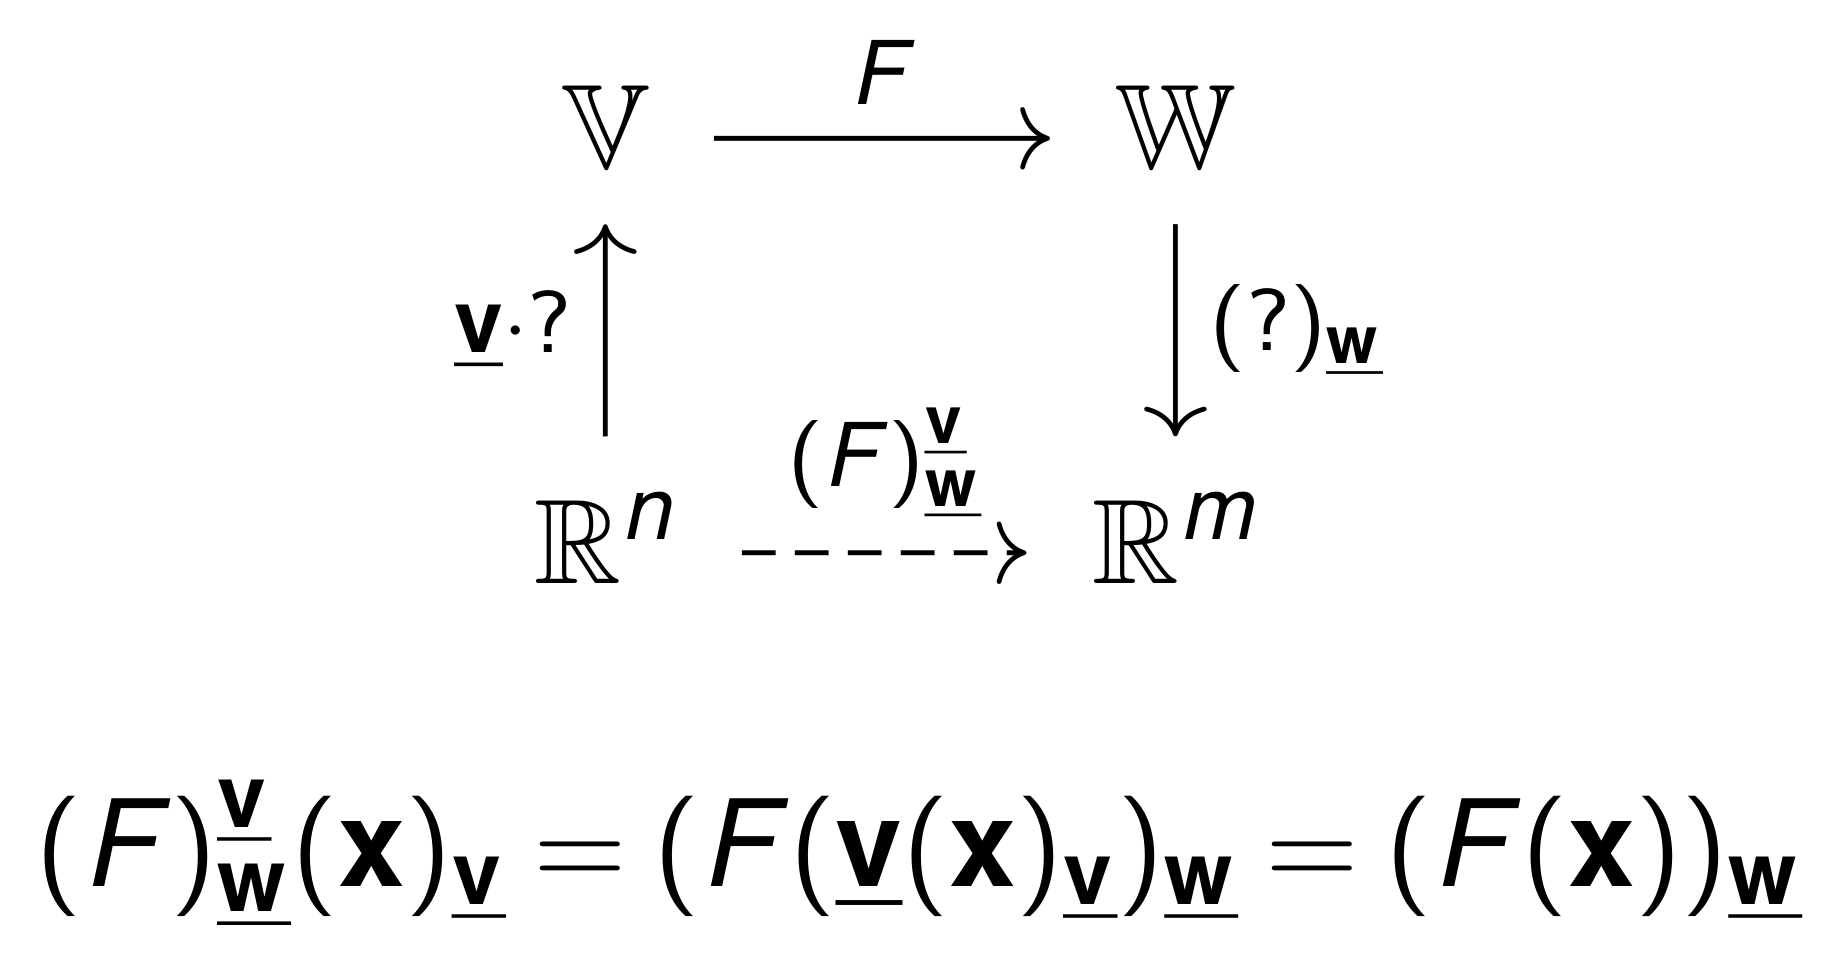
\includegraphics[width=8cm]{image/matris_lin_avb.png} 
    \caption{Matris av en linjär avbildning. From \cite{laII}}
\end{figure}

\textbf{Exempel: Rotations matrisen}
\begin{align*}
  &\left(\begin{array}{cc}
    \cos(\alpha) & -\sin(\alpha)   \\
    \sin(\alpha) &  \cos(\alpha)   \\
  \end{array}\right)  \\
  &\left(\begin{array}{ccc}
    1 & 0            & 0               \\
    0 & \cos(\alpha) & -\sin(\alpha)   \\
    0 & \sin(\alpha) &  \cos(\alpha)   \\
  \end{array}\right)
\end{align*}


%\textbf{Exempel: Derivatan av polynom}
%\begin{align*}
%  &\quad  \text{Bestäm matrisen för } \frac{d}{dx}\circ{G}:\mathbb{P}_2\to\mathbb{P}_2
%  \text{och } G\circ\frac{d}{dx}:\mathbb{P}_3\to\mathbb{P}_3 \\
%  &\quad \text{ där } \frac{d}{dx} \\
%  &\quad  G:\mathbb{P}_2\to\mathbb{P}_3 \text{ ges av } F(p(x))=(x+1)p(x) \\
%  &\quad  \frac{d}{dx}\circ{G}(a_0+a_1x+a_2x^2) = \frac{d}{dx}(x+1)(a_0+a_1x+a_2x^2) = \\
%  &\quad  \frac{d}{dx}(a_0 + (a_0+a_1)x + (a_1+a_2)x^2 + a_2x^3) =
%  a_0+a_1 + 2(a_1+a_2)x + 3a_2x^2 \\
%  &\quad  \text{Matrisn ska sltså sicka }
%  \begin{pmatrix} a_0 \\ a_1 \\ a_2 \end{pmatrix} \text{ på }
%  \begin{pmatrix} a_0+a_1 \\ 2a_1+2a_2 \\ 3a_2 \end{pmatrix} \text{ så }
%  {\big( \frac{d}{dx}\circ{G} \big)}^{w}_{w} =
%  \left(\begin{array}{ccc}
%    1 & 1 & 0  \\
%    0 & 2 & 2  \\
%    0 & 0 & 3  \\
%  \end{array}\right)  \\
%  &\quad
%  \left(\begin{array}{cccc}
%    0 & 1 & 0 & 0 \\
%    0 & 0 & 2 & 0 \\
%    0 & 0 & 0 & 3 \\
%  \end{array}\right) 
%  \left(\begin{array}{ccc}
%    1 & 0 & 0  \\
%    1 & 1 & 0  \\
%    0 & 1 & 1  \\
%    0 & 0 & 1  \\
%  \end{array}\right) =
%  \left(\begin{array}{ccc}
%    1 & 1 & 0  \\
%    0 & 2 & 2  \\
%    0 & 0 & 3  \\
%  \end{array}\right) 
%\end{align*}

\textbf{Exempel: Hitta matrisen}
\begin{align*}
  &\text{Linjär avbildning} F:\mathbb{P}_3\to\mathbb{P}_3, \, F= p+ p'+ p''+ p''' \\
  &\text{Ange $F$:s matris i standarbasen.} \\
  &\\
  &\text{Avbildar varge ellement i standardbasen } (1 \, x \, x^2 \, x^3) \\
  &F(1) = 1 + 1' + 1'' + 1''' = 1 \\
  &F(x) = x + x' + x'' + x''' = x+1 \\
  &F(x^2) = {x^2} + {x^2}' + {x^2}'' + {x^2}''' = x^2 + 2x + 2\cdot1 \\
  &F(x^3) = {x^3} + {x^3}' + {x^3}'' + {x^3}''' = x^3 + 3x^2 + 6x + 6\cdot1 \\
  &\left(\begin{array}{cccc}
    1 & 1 & 2 & 6 \\
    0 & 1 & 2 & 6 \\
    0 & 0 & 1 & 3 \\
    0 & 0 & 0 & 1 \\
  \end{array}\right)   
\end{align*}


\section{Basbyte av linjära avbildningar}
\textbf{Definition: Basbyte av linjära avblidningar}\par
låt $F: \mathbb{V}\to\mathbb{W}$ vara linjär. Låt $\underline{e}$ och
$\underline{v}$ vara baser i $\mathbb{V}$ och låt $\underline{f}$
och $\underline{w}$ vara baser av $\mathbb{W}$. Då gäller
${(F)}^{\underline{e}}_{\underline{f}}$ 
$=T^{\underline{w}}_{\underline{f}}{(F)}^{\underline{v}}_{\underline{w}}T^{\underline{e}}_{\underline{v}}$
Där vektorn kommer från höger (viktigt vid vilken ording transfomations matriserna står)

Ide: Vi omvandlar från en bas (ex standard bas) till en bas som
är mer anpasat för uträkningen.
Sedan omvandlar vi igen för att få svaret i den bas vi vill ha
den i (ex standard bas).

\textbf{Exempel: Basbyte av linjär avbildning vektor}
% q9 fråga 1

\textbf{Exempel: Basbyte av linjär avbildning polynom}
\begin{align*}
  &\text{Vad är matrisen av derivatan } \mathbb{P}_3\to\mathbb{P}_2 \\
  &\text{ med avseende på } \\
  &\text{basen } \underline{u} = (x^3 \, x^2 \, x \, 1) av \mathbb{P}_3 \text{ och }
  \underline{v} = (x^2 \, x \, 1)  \text{ av $\mathbb{P}_2$?}\\
  &\\
  &{(H)}^{\underline{e}}_{\underline{f}} =
  \left(\begin{array}{cccc}
    0 & 1 & 0 & 0 \\
    0 & 0 & 2 & 0 \\
    0 & 0 & 0 & 3 \\
  \end{array}\right)  \\
  &\\
  &T^{\underline{f}}_{\underline{v}}: \\
  &\vec{f}_1 = 1   = 0\vec{v}_1 + 0\vec{v}_2 + 1\vec{v}_3 \\
  &\vec{f}_2 = x   = 0\vec{v}_1 + 1\vec{v}_2 + 0\vec{v}_3 \\
  &\vec{f}_3 = x^2 = 1\vec{v}_1 + 0\vec{v}_2 + 0\vec{v}_3 \\
  &\\
  &T^{\underline{u}}_{\underline{e}}: \\
  &\vec{u}_1 = x^3 = 0\vec{e}_1 + 0\vec{e}_2 + 0\vec{e}_3 + 1\vec{e}_4 \\
  &\vec{u}_2 = x^2 = 0\vec{e}_1 + 0\vec{e}_2 + 1\vec{e}_3 + 0\vec{e}_4 \\
  &\vec{u}_3 = x   = 0\vec{e}_1 + 1\vec{e}_2 + 0\vec{e}_3 + 0\vec{e}_4 \\
  &\vec{u}_4 = 1   = 1\vec{e}_1 + 0\vec{e}_2 + 0\vec{e}_3 + 0\vec{e}_4 \\
  &\\
  &{(H)}^{\underline{u}}_{\underline{v}} =
  T^{\underline{f}}_{\underline{v}} {(H)}^{\underline{e}}_{\underline{f}} T^{\underline{u}}_{\underline{e}}= \\
  &\left(\begin{array}{ccc}
    0 & 0 & 1  \\
    0 & 1 & 0  \\
    1 & 0 & 0  \\
  \end{array}\right) 
  \left(\begin{array}{cccc}
    0 & 1 & 0 & 0 \\
    0 & 0 & 2 & 0 \\
    0 & 0 & 0 & 3 \\
  \end{array}\right) 
  \left(\begin{array}{cccc}
    0 & 0 & 0 & 1 \\
    0 & 0 & 1 & 0 \\
    0 & 1 & 0 & 0 \\
    1 & 0 & 0 & 0 \\
  \end{array}\right)  
\end{align*}



% normalisera

% avmilding matrisen är f^v_w om f:v \to w
% det är avbildingns matrisen om är i mitten av bassbyte formeln?

\section{Kärna och bild av en linjär avbildning}

\textbf{Definition: Kärna och bild}
\begin{align*}
  &\quad  \text{Låt $F:\mathbb{V}\to\mathbb{W}$ vara en linjär avbilding} \\
  &\quad  \\
  &\quad  \text{\textbf{Kärnan} eller \textbf{nollrummet} av den linjära avbildingen F} \\
  &\quad  \ker(F) = N(F) = \{\vec{v}\in\mathbb{V} | F(\vec{v} = \vec{0})\} \\
  &\quad  \\
  &\quad  \text{\textbf{Bilden} eller \text{värderummet} av den linjära avbildingen F} \\
  &\quad  \Ima(F) = V(F) = \{\vec{w}\in\mathbb{W} | \exists\vec{v}:F(\vec{v})=\vec{w}\} \\
\end{align*}

\textbf{Definition: Isomorfism, injektiv, surjektiv }
\begin{align*}
  &\quad  F:X\to{y} \text{ kallas} \\
  &\quad  \text{\textbf{injektiv} om } F(x) = F(x') \Rightarrow x = x' \\
  &\quad  \text{\textbf{surjektiv} om } \forall{y}\in Y\exists{x}\in{X}:f(x)=y \\
  &\quad  \text{\textbf{bijektiv} om det är både injektiv och surjektiv} 
\end{align*}

\textbf{Sats:}
\begin{align*}
  &\quad  \text{Låt $F:\mathbb{V}\to\mathbb{W}$ vara linjär} \\
  &\quad  F \text{ är injektiv omm } \ker{F} = \{\vec{0}\} \\
  &\quad  F \text{ är surjektiv omm } \Ima{F} = \mathbb{W} \text{ omm }
  \Rang ({(F)}^{\underline{u}}_{\underline{w}}) = \dim{\mathbb{W}} \\
\end{align*}


\textbf{Sats: Dimensionssatsen}
\begin{align*}
  &\quad  \text{För varje linjär avbilding $F:\mathbb{V}\to\mathbb{W}$ gäller} \\
  &\quad  \dim{\mathbb{V}} = \dim{\ker(F)} + \dim{\Ima(F)}  \\
\end{align*}

\textbf{Sats: Isomorfism}
\begin{align*}
  &\text{Låt $F:\mathbb{V}\to\mathbb{W}$ vara en linjär avbilding. De följande} \\
  &\text{är ekvivalenta}F \text{ är en isomorf} \\
  &\dim{\mathbb{V}} = \dim{\mathbb{W}} \text{ och $F$ är injektiva} \\
  &\dim{\mathbb{V}} = \dim{\mathbb{W}} \text{ och $F$ är surjektiva} \\
  &\det({(F)}^{\underline{v}}_{\underline{w}}) \neq 0 \\
  &{(F)}^{\underline{v}}_{\underline{w}} \text{ är en kvadratisk matris av rang }
  \dim{\mathbb{V}} = \dim{\mathbb{W}} \\
\end{align*}


% körna är att det finns en vektor som ablidast till noll vektorn
% dim ker(f) = antal fria variabler
% dim im(f) = antal priof elementen


\section{Egenvärden och egenvektorer}
% definition
\textbf{Definition: Egenvärde och egenvektor}
Låt $F:\mathbb{V}\to\mathbb{W}$ vara en linjär avbilding.
En vektor $\vec{v}\neq\vec{0}$ kallas en egenvektor till $F$ om det finns $\lambda\in\mathbb{R}$ så att
$F(\vec{v}) = \lambda\vec{v}$
I detta fall kallas $\lambda$ en \textbf{egenvärde} till $F$
$\mathbb{V}_{F,\lambda} = \{ \vec{v}\in\mathbb{V} | F(\vec{v}) = \lambda\vec{v} \}$
kallas \textbf{egenrummet} av $F$ till egenvärdet $\lambda$

% seculärpolynomet
\textbf{Definition: Sekularpolynomet}
För en matris $A$ kallas polynomet $\chi_A(\lambda) = \det(A-\lambda I_n)$
\textbf{sekularpolynomet} till $A$
Om $A= {(F)}^{\underline{e}}_{\underline{e}}$, så kallas $\chi_A$ också
sekularpolunomet till $F$.

% ett huvud exempel står i notes
\textbf{Exempel:}
\begin{align*}
  &F:\mathbb{R}^3\to\mathbb{R}^3 \text{ matrisen i standardbasen är} \\
  &\left(\begin{array}{ccc}
    1 & 2 & 2  \\
    0 & 2 & 1  \\
   -1 & 2 & 2  \\
  \end{array}\right) \\
  &\\
  &\text{1. Hittar egenvärderna} \\
  &F (\vec{x}) = \lambda\vec{x} \Leftrightarrow{} A\vec{x}=\lambda\vec{x} \\
  &A\vec{x}-\lambda\vec{x} = \vec{0} \Leftrightarrow{} (A-\lambda{I})\vec{x} = 0 \\
  &\text{Där $\lambda$ är egenvärdet, och $\vec{x}$ är egenvektorn} \\
  &A-\lambda{I} =
  \left(\begin{array}{ccc}
    1-\lambda & 2         & 2          \\
    0         & 2-\lambda & 1          \\
   -1         & 2         & 2-\lambda  \\
  \end{array}\right) \\
  &\det(A-\lambda{I}) = 4 -2\lambda{} -(2 -\lambda)(4 -3\lambda+\lambda^2) \\
  &= (2-\lambda)(-2 +3\lambda -\lambda^2) \\
  &\det(A-\lambda{I}) = 0 \Leftrightarrow{} \lambda=2 \lor{} \lambda=1 \\
  &\\
  &\text{2. Hittar egenvektorerna} \\
  &\lambda=2: \\
  &(A-2I)\vec{x} \Leftrightarrow{}
  \left(\begin{array}{ccc|c}
    1-2 & 2   & 2   & 0 \\
    0   & 2-2 & 1   & 0 \\
   -1   & 2   & 2-2 & 0 \\
  \end{array}\right) \\
  &\sim{}
  \left(\begin{array}{ccc|c}
    1 & -2 & 0 & 0 \\
    0 &  0 & 1 & 0 \\
    0 &  0 & 0 & 0 \\
  \end{array}\right) \\
  &\quad \Leftrightarrow{}
  \begin{pmatrix} x_1 \\ x_2 \\ x_3 \end{pmatrix} =
  \begin{pmatrix} 2t \\ t \\ 0 \end{pmatrix} =
  t\begin{pmatrix} 2 \\ 1 \\ 0 \end{pmatrix}, \, t\in\mathbb{R} \\
  &\quad \text{Så egenrummet till $\lambda=2$ är linjära höljet: }
  \Big[ \begin{pmatrix} 2 \\ 1 \\ 0 \end{pmatrix} \Big]  \\
  &\quad  \\
  &\quad  \lambda=1: \\
  &\quad  (A-1I)\vec{x} \Leftrightarrow{}
  \left(\begin{array}{ccc|c}
    1-1 & 2   & 2   & 0 \\
    0   & 2-1 & 1   & 0 \\
   -1   & 2   & 2-1 & 0 \\
  \end{array}\right) \\
  &\sim{}
  \left(\begin{array}{ccc|c}
    1 &  0 & 1 & 0 \\
    0 &  1 & 1 & 0 \\
    0 &  0 & 0 & 0 \\
  \end{array}\right) \\
  &\quad \Leftrightarrow{}
  \begin{pmatrix} x_1 \\ x_2 \\ x_3 \end{pmatrix} =
  \begin{pmatrix} -t \\ -t \\ t \end{pmatrix} =
  t\begin{pmatrix} -1 \\ -1 \\ 1 \end{pmatrix}, \, t\in\mathbb{R} \\
  &\quad \text{Så egenrummet till $\lambda=1$ är linjära höljet: } \\
  &\Big[ \begin{pmatrix} -1 \\ -1 \\ 1 \end{pmatrix} \Big]  \\
\end{align*}


\section{Diagonalisering}
\textbf{Definition: Diagonalisering}
Låt $F:\mathbb{V}\to\mathbb{V}$ vara en linjär avbildning. Då kallas $F$
\textbf{diagonaliserbar} om det finns en bas $\underline{v}$ som består av
egenvektorer till $F$. 
(Det betyder att ${(F)}^{\underline{v}}_{\underline{v}}$ är en diagonalmatris).

% algebraisk och gemotrisk multiplicitet
\textbf{Definition: Algebraisk och Geometrisk multiplicitet}
\textbf{Algebraisk multiplicitetet} av en egenvärde $\lambda_0$ till en
matris $A$ är det maximala talet $m$, så att
$\chi_A(\lambda) = {(\lambda-\lambda_0)}^m p(\lambda)$ för någon polunom $p$.

\textbf{Algebraisk multiplicitetet} av en egenvärde $\lambda_0$ till en
matris $A$ är $\dim{\mathbb{V}_{A,\lambda_0}}$.

\textbf{Exempel: }
\begin{align*}
  &\text{Avför om matrisen är diagoniserbar och} \\
  &\text{isåfal vad är den matrisen} \\
  &M = 
  \left(\begin{array}{ccc}
   -2 & 4 & 4  \\
    0 & 2 & 4  \\
    0 & 0 & -2 \\
  \end{array}\right) \\
  &\\
  &\text{1. Hittar egenvärden:} \\
  &\text{(se i kaptlet om enhetsvektorer) } \\
  &(-2-\lambda)(2-\lambda)(-2-\lambda)=0 \\
  &\lambda=2 \text{ (alg mult 1) } \lor{} \lambda=-2 \text{ (alg mult 2) } \\
  &\\
  &\text{2. Hittar egenvekorer:} \\
  &\text{(se i kaptlet om enhetsvektorer) } \\
  &\lambda=2 \Leftrightarrow{}
  \begin{pmatrix} x_1 \\ x_2 \\ x_3 \end{pmatrix} =
  \begin{pmatrix} t \\ t \\ 0 \end{pmatrix} =
  t\begin{pmatrix} 1 \\ 1 \\ 0 \end{pmatrix}, \, t\in\mathbb{R} \\
  &\text{geo mult 1 därmed så är den hittils diagonaliserbar } \\
  &\\
  &\lambda=-2 \Leftrightarrow{}
  \begin{pmatrix} x_1 \\ x_2 \\ x_3 \end{pmatrix} =
  \begin{pmatrix} s \\ -t \\ t \end{pmatrix} \\
  &=s\begin{pmatrix} 1 \\ 0 \\ 0 \end{pmatrix} +
  t\begin{pmatrix} 0 \\ -1 \\ 1 \end{pmatrix}, \, s,t\in\mathbb{R} \\
  &\text{geo mult 2 därmed diagonaliserbar } \\
  &\\
  &\text{3. Sätter upp diagonala matrisen} \\
  &{F}^{\underline{e}}_{\underline{e}} =
  {T}^{\underline{v}}_{\underline{e}} {F}^{\underline{v}}_{\underline{v}} {T}^{\underline{e}}_{\underline{v}}
  \Leftrightarrow{} 
  \left(\begin{array}{ccc}
   -2 & 4 & 4  \\
    0 & 2 & 4  \\
    0 & 0 & -2 \\
  \end{array}\right) = \\
  &\left(\begin{array}{ccc}
    1 & 1 &  0  \\
    1 & 0 & -1  \\
    0 & 0 &  1  \\
  \end{array}\right)
  \left(\begin{array}{ccc}
    2 &  0 &  0  \\
    0 & -2 &  0  \\
    0 &  0 & -2 \\
  \end{array}\right)
  \left(\begin{array}{ccc}
    1 & 1 &  0 \\
    1 & 0 & -1 \\
    0 & 0 &  1 \\
  \end{array}\right)^{-1} \\
\end{align*}


\section{Inre produkrum}
% egenskaper för skalär produkt
\textbf{Definition: Skalärprodukt}
Låt $\mathbb{V}$ vara ett vektorrum. En \textbf{skalärprodukt} på $\mathbb{V}$ är
en operation som tillordnar varge par av vketorer $\vec{u},\vec{v}\in\mathbb{V}$ en skalär
$(\vec{u}|\vec{v})\in\mathbb{R}$ så att följade vilkor gäller:
bilinjär
\begin{enumerate}
  \item $(\vec{u} + \vec{v}|\vec{w}) = (\vec{u}|\vec{w}) + (\vec{v}|\vec{w})$
  \item Symetrisk $(\lambda\vec{u}|\vec{v}) = \lambda(\vec{u}|\vec{v}) = (\vec{u}|\lambda\vec{v})$
  \item Positiv definit $(\vec{u}|\vec{v}) = (\vec{v}|\vec{u})$
  \item Om $\vec{u}\neq\vec{0}$ så $(\vec{u}|\vec{u}) > 0$
\end{enumerate}

\textbf{Definition: Avstånd och vinklar}
Låt $\mathbb{V}$ vara ett vektorrum med enskalärprodukt och $\vec{u},\vec{v}\in\mathbb{V}$
\begin{enumerate}
  \item Längden (normen) av $\vec{u}$ betecknas $|\vec{u}|$ och defineras som $|\vec{u}|=\sqrt{\vec{u}|\vec{u}}$.
  \item Avstånder mellan $\vec{u}$ och $\vec{v}$ defineras som $\vec{u}-\vec{v}$
  \item Om $\vec{u}\neq{0}$ och $\vec{v}\neq{0}$ defineras vinkeln mellan
    $\vec{u}$ och $\vec{v}$ som
    $\cos^{-1}\frac{(\vec{u}|\vec{v})}{|\vec{u}||\vec{v}|}$
  \item Vi säger att $\vec{u}$ och $\vec{v}$ är ortogonala om
    $(\vec{u}|\vec{v})=0$
\end{enumerate}

\textbf{Definition: Trianglar}
\begin{align*}
  &\text{Lår $\mathbb{V}$ vara ett vektorrum med en} \\
  &\text{skalärprodukt och} \vec{u},\vec{v}\in\mathbb{V} \\
  &\text{Då bildar $\vec{u},\vec{b}$ och $\vec{u}+\vec{v}$ en triangel} \\
  &{|\vec{u}+\vec{v}|}^2 = {|\vec{u}|}^2 + {|\vec{v}|}^2 + 2(\vec{u}|\vec{v}) \\
\end{align*}

\textbf{Definition: Ortogonal projektion och komponent}
\begin{enumerate}
  \item 1. $\vec{u}_{\|\vec{u}} := \frac{(\vec{v}|\vec{u})}{(\vec{u}|\vec{u})}\vec{u}$
    kallas den ortogonala projektionen av $\vec{v}$ på $\vec{u}$.
  \item 2. $\vec{u}_{\perp{\vec{u}}} := \vec{v} - \vec{v}_{\|\vec{u}}$
    kallas den ortogonala kompnenten av $\vec{v}$ med avseende på $\vec{v}$.
\end{enumerate}


\section{Symetriska och positiva definita matriser}
\textbf{Formel: skalärprodukt utrykt med matriser}
$(\vec{u}|\vec{y}) = \vec{u}^t A \vec{y}$
där $A$ är $(n \times n)$-matrisen som uppfyller följande krav:
\begin{enumerate}
  \item Symetrisk om $A^t=A$.
  \item Positivt definit om $\vec{x}^t A \vec{x} > 0, \, \forall \vec{x}\in\mathbb{R}^n, \, \vec{x}\neq \vec{0}$.
\end{enumerate}

% Exempel: hurman visar att det är en skalärprodukt
\textbf{Exempel: skalärprodukt utrykt med matriser}
\begin{align*}
  &\text{På $\mathbb{R}^2$ definierar vi } \\
  &(\vec{x}|\vec{y}) = x_1y_1 + 3x_1y_2 + ax_2y_1 + bx_2y_2 \\
  &\text{För vilka värdenpå $a$ och $b$ är detta en} \\
  &\text{skalärprodukt? } a,b \in \mathbb{R} \\
  &\\
  &\text{Lösn: } \\
  &\text{1. Symetrisk:  }  (\vec{x}|\vec{y}) = (\vec{y}|\vec{x}) \\
  &= y_1x_1 + 3y_1x_2 + ay_2x_1 + by_2x_2 \\
  &(\vec{x}|\vec{y}) =
  \vec{x}^t
  \left(\begin{array}{cc}
    1 & 3 \\
    a & b \\
  \end{array}\right)
  \vec{y} \Rightarrow{a=3} \text{pga summetri} \\
  &\\
  &\text{2. Pos def:  }  (\vec{x}|\vec{x}) > 0, \, \forall{} \vec{x} \neq{\vec{0}}  \\
  &(\vec{x}|\vec{x}) = (x_1 x_2)
  \left(\begin{array}{cc}
    1 & 3 \\
    a & b \\
  \end{array}\right) \begin{pmatrix} x_1 \\ x_2 \end{pmatrix} \\
  &= {x_1}^2 + 3x_1x_2 + 3x_2+x_1 + b{x_2}^2 \\
  &= {x_1}^2 + 6x_1x_2 + b{x_2}^2 = {(x_1+3x_2)}^2 + (b-9){x_2}^2 \\
  &\text{vilket endast är positivt då } b>9 \\
\end{align*}


\section{On-baser och Gram-Schmidt-ortonormalisering}
\textbf{Definition: ON-bas}
\begin{align*}
  &\text{Låt $\mathbb{V}$ vara ett vektorrum med en skalärprodukt. } \\
  &\text{En mängd $\{ \vec{u_1} \ldots \vec{u_n} \} \subseteq \mathbb{V}$ kallas ortonormal} \\
  &\text{(ON) om} \\
  &(\vec{u_i}|\vec{u_j}) = 
  \left\{\begin{array}{rr}
  1 \, i = j \\
  0 \, i \neq i  \\
  \end{array}\right. \\
  &|\vec{u_i}| = 1 \\
  &\\
  &\text{Dvs alla vektorer är ortogonala mot varandra} \\
  &\text{och att längden ska vara $1$} \\
\end{align*}

\textbf{Definition: Koordinater i en ON-bas}
\begin{align*}
  &\text{Låt $\underline{u} = (\vec{u_1} \ldots \vec{u_n})$ vara en ON-bas i $\mathbb{V}$ och } \\
  &\vec{v}, \vec{w} \in\mathbb{V} \text{ Då är} \\
  &\text{1. } \vec{v}_{\underline{u}} =
  \begin{pmatrix} (\vec{v}|\vec{u}_1) \\ . \\ . \\ (\vec{v}|\vec{u}_n) \end{pmatrix} \\
  &\text{2. } (\vec{v}|\vec{w}) =
  (\vec{v}|\vec{u}_1)(\vec{w}|\vec{u}_1)+ \ldots +(\vec{v}|\vec{u}_n)(\vec{w}|\vec{u}_n) \\
  &= \vec{v}_n \bullet \vec{w}_n \\
\end{align*}

\textbf{Definition: Ortogonal komplement}
Låt $\mathbb{V}$ vara ett vektorrum med en skalärprodukt och
$\mathbb{U} \subseteq \mathbb{V}$ ett underrum. Då är
$\mathbb{U}^{\perp} = \{ \vec{v}\in\mathbb{V} | (\vec{u}|\vec{v}) = 0, \, \forall \vec{u} \in \mathbb{U} \}$
ett underrum som kallas det ortogonala koplementet till $\mathbb{U}$.

\textbf{Exempel: Hitta en ON-bas med Gram-Schidt ortonormalisering}
\begin{align*}
  &U = [\vec{u}_1, \vec{u}_2, \vec{u}_3] \subseteq \mathbb{R}^4 , \,
  \vec{u}_1 = \begin{pmatrix} 1 \\ 1 \\ 1 \\ 0 \end{pmatrix}
  \vec{u}_2 = \begin{pmatrix} 1 \\ 0 \\ 2 \\ 1 \end{pmatrix}
  \vec{u}_3 = \begin{pmatrix} 0 \\ 0 \\ 1 \\ 1 \end{pmatrix} \\
  &\text{Hitta ON-bas} \\
  &\\
  &[\vec{u}_1] \subseteq [\vec{u}_1, \vec{u}_2] \subseteq [\vec{u}_1, \vec{u}_2, \vec{u}_3] \\
  &\text{där } [\vec{u}_1] = U_1, \, [\vec{u}_1, \vec{u}_2] = U_2, \, [\vec{u}_1, \vec{u}_2, \vec{u}_3] = U_3
  &\\
  &\text{ON-bas } U_1: f_1 = \frac{1}{|\vec{u_1}|} \vec{u_1} =
  \frac{1}{\sqrt{3}}\begin{pmatrix} 1 \\ 1 \\ 1 \\ 0 \end{pmatrix}  \\
  &\\
  &\text{ON-bas } U_2: f_1,f_2 \, \vec{u}_{2\perp\vec{u_1}} = \vec{u_2} - (\vec{u_2}|f_1)f_1 \\
  &= \begin{pmatrix} 1 \\ 0 \\ 2 \\ 1 \end{pmatrix} -
  \frac{1}{\sqrt{3}}(1+0+2+0)\frac{1}{\sqrt{3}}\begin{pmatrix} 1 \\ 1 \\ 1 \\ 0 \end{pmatrix} \\
  &= \begin{pmatrix} 0 \\ -1 \\ 1 \\ 1 \end{pmatrix} \\
  &f_2 = \frac{1}{\vec{u}_{2\perp\vec{u_1}}}\vec{u}_{2\perp\vec{u_1}} 
  = \frac{1}{\sqrt{3}}\begin{pmatrix} 0 \\ -1 \\ 1 \\ 1 \end{pmatrix}  \\
  &\\
  &\text{ON-bas } U_3: f_1,f_2,f_3 \, \vec{u}_{3\perp\vec{u_2}}
  = \vec{u_3} - (\vec{u_3}|f_1)f_1 - (\vec{u_3}|f_2)f_2 \\
  &= \begin{pmatrix} 0 \\ 0 \\ 1 \\ 1 \end{pmatrix}
  - \frac{1}{\sqrt{3}}(0+0+1+0)\frac{1}{\sqrt{3}}\begin{pmatrix} 1 \\ 1 \\ 1 \\ 0 \end{pmatrix} \\
  &- \frac{1}{\sqrt{3}}(0+0+1+1)\frac{1}{\sqrt{3}}\begin{pmatrix} 0 \\ -1 \\ 1 \\ 1 \end{pmatrix} \\
  &=  \begin{pmatrix} 0 \\ 0 \\ 1 \\ 1 \end{pmatrix}
  - \frac{1}{3}\begin{pmatrix} 1 \\ 1 \\ 1 \\ 0 \end{pmatrix}
  - \frac{2}{3}\begin{pmatrix} 1 \\ 1 \\ 1 \\ 0 \end{pmatrix}
  = \frac{1}{3}\begin{pmatrix} -1 \\ 1 \\ 0 \\ 1 \end{pmatrix} \\
  &\Rightarrow  f_3 = \frac{1}{\sqrt{3}}\begin{pmatrix} -1 \\ 1 \\ 0 \\ 1 \end{pmatrix} \\
  &\\
  &\text{Kontrollera att $f_1, f_2, f_3$ är ortogonala mot varandra} \\
\end{align*}


\section{Isometriska avbildningar och spektralsatsen}
\textbf{Definition: isometrier}
\begin{align*}
  &\quad  \text{Låt $\mathbb{V}$ och $\mathbb{W}$ vara vektorrum med skalärprodukter. } \\
  &\quad  \text{En linjär avbilding} \\
  &\quad  F:\mathbb{V}\to\mathbb{W} \\
  &\quad  \text{kallas en isomerik om } |F(\vec{v})| = |\vec{v}| \\
  &\quad  \text{En isometrisk linjär avbildling kallas också en isometri.} \\
  &\quad  \\
  &\quad  \text{dvs. Så är längden oförendrad. $F$ är en isometri omm } \\
  &\quad  (F(\vec{u})|F(\vec{v})) = (\vec{u}|\vec{u}) \\
\end{align*}

\textbf{Egenskaper: isometrier}
\begin{align*}
  &\text{\textbf{Sats:} Låt $F:\mathbb{V}\to\mathbb{W}$ vara en isometri. Då är $F$} \\
  &\text{injektiv} \\
  &\text{\textbf{Sats:} Låt $F:\mathbb{V}\to\mathbb{W}$ vara en iventerbar isometri.} \\
  &\text{Då är $F^{-1}:\mathbb{W}\to\mathbb{V}$ en isometri} \\
  &\text{\textbf{Sats:} Låt $F:\mathbb{U}\to\mathbb{V}$ och $G:\mathbb{V}\to\mathbb{W}$ vara en} \\
  &\text{isometrier. Då är $G\circ{F}:\mathbb{U}\to\mathbb{W}$ en isometri} \\
\end{align*}

\textbf{Sats: spektralsatsen}
Låt $\mathbb{V}$ vara ett ändligt dimensionellt vektorrum med en
skalär produkt och $F:\mathbb{V}\to\mathbb{V}$ en linjär avbildining.
Då är följande vilkor ekvivalenta
\begin{enumerate}
  \item $F$ är symmetrisk.
  \item $\mathbb{V}$ har en ON-bas av bestående av egenvektorer till $F$.
\end{enumerate}

Låt $A$ vara en $(n\times{n})$-matris. Då är följande vilkor ekvivalenta
\begin{enumerate}
  \item $A$ är symmetrisk.
  \item Det finns en ortonormal matris $T$ så att $D=T^{-1}AT$ är en diagonalmatris.
\end{enumerate}


\section{Andragradskurvor och andragradsytor}
\begin{align*}
  &\quad  Q(x)=1
  \Leftrightarrow 1 x^t A x = 1
  \Leftrightarrow y^t D y = 1 \\
  &\Leftrightarrow \lambda_1 {y_1}^2 + \lambda_2 {y_2}^2 = 1 \\
  &\\
  &\text{Om $\lambda_1 = \lambda_2$ så berkriver $Q(x)=1$ en cirkel} \\
  &\text{Om $\lambda_1 > 0$ och $\lambda_2 > 0$ så berkriver $Q(x)=1$} \\
  &\text{en ellips} \\
  &\text{Om $\lambda_1 > 0$ och $\lambda_2 < 0$ så berkriver $Q(x)=1$} \\
  &\text{en hyperbel} \\
\end{align*}

\textbf{Exempel: Bestäm formen}
\begin{align*}
  &Q(\vec{x})= \frac{14}{5}{x_1}^2 +  \frac{11}{5}{x_2}^2 + \frac{14}{5}x_1x_2  \\
  &\\
  &Q(\vec{x}) = (x_1 \, x_2 )
  \left(\begin{array}{cc}
    14/5 &  2/5  \\
     2/5 & 11/5  \\
  \end{array}\right) \begin{pmatrix} x_1 \\ x_2 \\ \end{pmatrix} \\
  &\text{1. Egenvärden} \det{A} = (\frac{14}{5} -\lambda) (\frac{11}{5} -\lambda) -\frac{4}{25} \\
  &= 0 \\
  &\lambda_1 = 2 > 0 \\
  &\lambda_2 = 3 > 0 \\
  &\text{Därmed så beskriver $Q(x)=1$ en ellips} \\
  &\text{2. Egenvektor får vi en ON-bas} \\
  &\text{3. Ställer up ekvationen och ritar ut den} \\
  &Q (\vec{y}) = y^-1
  \left(\begin{array}{cc}
    2 & 0  \\
    0 & 3  \\
  \end{array}\right) \vec{y} = 2{y_1}^2 + 3{y_2}^2 = 1
\end{align*}


\section{System av linjära differentialekvationer}
\begin{align*}
  &\quad  y'=Ay \\
  &\quad  T^{-1}AT=D \\
  &\quad  y=Tz \Rightarrow y'=Tz' \land y'=Ay \Leftrightarrow z'=dz \\
  &\quad  z=
  \begin{pmatrix} c_1e^{\lambda_1t} \\ c_2e^{\lambda_2t} \\.\\.\\.\\ c_n e^{\lambda_n t} \end{pmatrix}
  \text{ där } c_i\in\mathbb{R}^n  \text{ och } y=Tz \\
  &\quad  c = T^{-1}y_0 \text{ där } z(0) = c =
    \begin{pmatrix} c_1 \\.\\.\\.\\ c_n \end{pmatrix} 
\end{align*}

\textbf{Exempel: Bestäm formen}
\begin{align*}
  &\text{Lös följade system av differentialekvationer} \\
  &\left\{\begin{array}{rrr}
  \frac{dx(t)}{dt} = 2x(t) + y(t) + z(t) \\
  \frac{dy(t)}{dt} =  x(t) +2y(t) + z(t) \\
  \frac{dz(t)}{dt} =  x(t) + y(t) +2z(t) \\
  \end{array}\right. x (0) =3, \, y (0) =2, \, z (0) =1  \\
  &\\
  &\text{1. Skriver up systemet} \\
  &
  \begin{pmatrix} \frac{dx (t)}{dt} \\ \frac{dy (t)}{dt} \\ \frac{dz (t)}{dt} \end{pmatrix} =
  \left(\begin{array}{ccc}
    2 & 1 & 1 \\
    1 & 2 & 1 \\
    1 & 1 & 2 \\
  \end{array}\right)
  \begin{pmatrix} x (t) \\ y (t) \\ z (t)  \end{pmatrix}  \text{ Där matrisen är $A$} \\
  &\\
  &\text{2. Diagonaliserar} \\
  &\text{2.1 egenvärden} \\
  &\lambda_1 = 1 \text{ (multiplicitet 2), } \lambda_2 = 4 \text{ (multiplicitet 1) } \\
  &\text{2.1 egenvektor} \\
  &\lambda_1 = 1 \Rightarrow{}  A -I =
  \left(\begin{array}{ccc}
    1 & 1 & 1 \\
    1 & 1 & 1 \\
    1 & 1 & 1 \\
  \end{array}\right)  \\
  &\Rightarrow{}
  \vec{v}_1 = \begin{pmatrix} 1 \\ 0 \\ -1  \end{pmatrix} \land{}
  \vec{v}_2 = \begin{pmatrix} 0 \\ 1 \\ -1  \end{pmatrix} \\
  &\lambda_2 = 4 \Rightarrow{}  A -4I =
  \left(\begin{array}{ccc}
    -2 & 1 & 1 \\
    1 & -2 & 1 \\
    1 & 1 & -2 \\
  \end{array}\right) \Rightarrow{}
  \vec{v}_3 = \begin{pmatrix} 1 \\ 1 \\ 1  \end{pmatrix} \\
  &\text{Diagonal ekv blir } A=TDT^-1 \\
  &\Rightarrow{} T =
  \left(\begin{array}{ccc}
    1 &  0 & 1 \\
    0 &  1 & 1 \\
    -1 & -1 & 1 \\
  \end{array}\right) \, \land{} \, D =
  \left(\begin{array}{ccc}
    1 & 0 & 0 \\
    0 & 1 & 0 \\
    0 & 0 & 4 \\
  \end{array}\right)
  &\\
  &\text{3. Finner den almäna lösningen} \\
  &u'=Du \Rightarrow{}
  \left\{\begin{array}{rrr}
  u_1 = c_1e^{t} \\
  u_2 = c_2e^{t} \\
  u_3 = c_3e^{4t} \\
  \end{array}\right. \text{ Där } c_1,c_2,c_3\in\mathbb{R} \\
  &v'=Av \text{ Där } A^{-1}v' = Tu \Rightarrow{} v=Tu \\
  &v = \begin{pmatrix} x(t) \\ y(t) \\ z(t)  \end{pmatrix} = 
  \left(\begin{array}{ccc}
    1 &  0 & 1 \\
    0 &  1 & 1 \\
    -1 & -1 & 1 \\
  \end{array}\right) \begin{pmatrix} c_1e^{t} \\ c_2e^{t} \\ c_3e^{4t} \end{pmatrix} \\
  &=\begin{pmatrix} c_1e^{t} + c_2e^{t} \\ c_2e^{t} + c_3e^{4t} \\ -c_1e^{t} -c_2e^{t} +c_3e^{4t} \end{pmatrix} \\
  &\\
  &\text{4. Finner lösningen till begynelsevärdet} \\
  &
  \left(\begin{array}{ccc|c}
    1  &  0 & 1 & 3 \\
    0  &  1 & 1 & 2 \\
    -1 & -1 & 1 & 1 \\
  \end{array}\right) \sim{}
  \left(\begin{array}{ccc|c}
    1  &  0 & 0 & 1 \\
    0  &  1 & 0 & 0 \\
    0  &  0 & 1 & 2 \\
  \end{array}\right) \Rightarrow{}
  \begin{pmatrix} c_1 \\ c_2 \\ c_3 \end{pmatrix} =
  \begin{pmatrix} 1 \\ 0 \\ 2 \end{pmatrix}  \\
  &\left\{\begin{array}{rrr}
  x (t) = e^t + 2e^{4t} \\
  y (t) = 2e^{4t} \\
  z (t) = -e{t} + 2e^{4t} \\
  \end{array}\right. \\
\end{align*}
\end{multicols}
\raggedcolumns